\normaltrue
\correctionfalse

%\UPSTIidClasse{12} % 11 sup, 12 spé
%\newcommand{\UPSTIidClasse}{12}

\exer{Question de cours -- Torsion $\star$ \label{RDM:03:tor:539:cours}}
\setcounter{question}{0}\marginnote{\xpComp{RDM}{03}}%\UPSTIcompetence[2]{C2-10}
\index{Compétence RDM-03}



\ifcorrection
\else
\marginnote{\textbf{Pas de corrigé pour cet exercice.}}
\fi


\question{Donner la définition de la contrainte en torsion, la relation entre la contrainte et déformation, et la relation entre effort et déformation. }

\ifprof
$\tau = \dfrac{M_t}{I_G}r$, $\tau = G r \gamma_x$, $M_t= G \gamma_x I_G$ et $\Delta \theta_x = \gamma_x L$.
\else
\fi

\question{Donner la défintion du moment quadratique polaire. Calculer $I_G(S)$ pour une poutre creuse de section circulaire (grand rayon $R$ et petit rayon $r$).}

\ifprof
On a $\int_G(S)=\int_S r^2 \dd S$.

Pour un cylindre plein : on a $I_G(S)=\dfrac{\pi D^4}{32} = \dfrac{\pi R^4}{2}$.
Pour une poutre creuse : $I_G(S) = \dfrac{\pi \left(R^4 -r^4\right) }{2} $.
\else
\fi

\question{Tracer le champ de contrainte dans chacune des deux sections. }
\ifprof
\else
\fi


\begin{marginfigure}
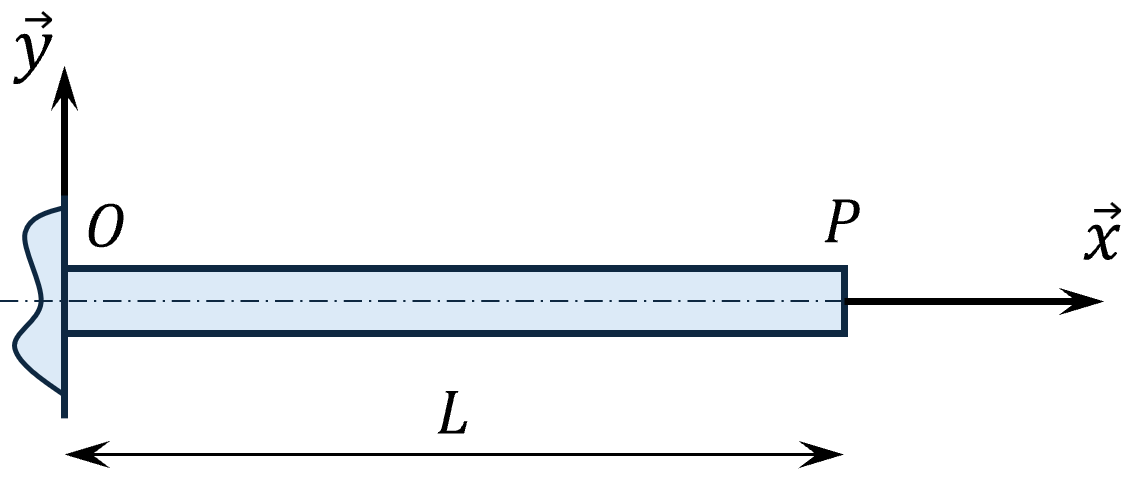
\includegraphics[width=\linewidth]{539_01.png}
\end{marginfigure}
Soit la barre de torsion ci-contre encastrée en $O$. On a $\vectm{P}{\text{ext}}{\text{poutre}} = C\vect{x}$. On donne $C = \SI{10}{Nm}$, $D=\SI{10}{mm}$ et $L=\SI{100}{mm}$.

\question{Déterminer la contrainte tangentielle maximale au sein de la poutre.}
\ifprof
\else
\fi

\question{Déteminer l'angle de torsion entre le poit $O$ et le point $P$.}

\ifprof
L'angle unitaire de torsion est donné par $\gamma_x = \dfrac{M_t }{GI_G}$ avec $G=\dfrac{E}{2(1+\nu)}$.

AN : 
$E = \SI{200 000}{MPa}$ et $\nu = 1$, alors $G = \SI{77 0000}{MPa}$
$I_{G_p} = \dfrac{\pi 5^4}{2} = \SI{981}{mm^4}$ 

$\gamma_x = \dfrac{M_t }{I_G G} = \dfrac{10 000}{77 000\times 981} = \SI{1,3e-4}{rad}$




\else
\fi

\question{Déteminer l'angle de torsion entre le poit $O$ et le point $P$ pour une barre creuse dont le diamètre intérieur est de \SI{5}{mm}.}
\ifprof
\else
\fi


\question{Donner la différence de masse, de contrainte et d'angle de torsion entre les deux barres.}
\ifprof
\else
\fi


\ifprof

\else
%\footnotesize
%\begin{enumerate}
%  \item $\left(fp + Mp^2\right) Z(p)=S_h P_h(p)-S_e P_e(p) - \dfrac{Mg}{p}$
%    \item $Q_e(p)=\left(S_a - S_b \right)pL(p) + \dfrac{V_t}{B_e} p P_e(p)$ et $mp^2 L(p) = -rL(p)+\left(S_a-S_b\right) P_e(t)-f'pL(p)$.
%\end{enumerate}
%\normalsize

\marginnote{Corrigé voir \ref{RDM:02:trac:539:cours}.}

\fi